\documentclass[12pt]{scrreprt}
\usepackage[utf8]{inputenc}
\usepackage[ngerman]{babel}
\usepackage[utf8]{inputenc}
\usepackage[T1]{fontenc}
\usepackage{hyperref}
%\hypersetup{colorlinks=true, citecolor=red}

\usepackage{natbib}
\usepackage[numbib]{tocbibind}
\usepackage{float}
\linespread{1.3}
\usepackage{natbib}
\usepackage{graphicx}
\usepackage{pdfpages}
\usepackage[euler]{textgreek}
\usepackage{adjustbox}
\usepackage[margin = 3cm]{geometry}


\usepackage{eso-pic} 
\usepackage{lipsum} 

\usepackage{tabularx} 
\usepackage{multirow}
\usepackage{amssymb}
\usepackage[flushleft]{threeparttable}
\usepackage{booktabs,caption}

\usepackage{amsmath}


\pagenumbering{roman}
\begin{document}
	\pagestyle{myheadings}
	
	
	
	
	
\begin{titlepage}
\begin{center}
\begin{minipage}{0.6\textwidth}%
\begin{flushleft}
					Ludwig-Maximilians-Universität \\
					Institut für Statistik \\
					Wintersemester 2019/2020 \\
					
\end{flushleft}
\end{minipage}
\begin{minipage}{0.35\textwidth}%
	\begin{flushright}
	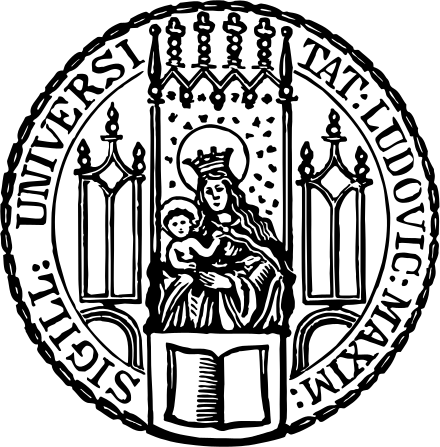
\includegraphics[scale = 0.25]{bilder/lmu_logo}
\end{flushright}
	\end{minipage}%
	\end{center}
		
		
		
		\vspace{4cm}
		{\centering
			
			{
				\Large\bfseries Abschlussbericht zum Projekt\\
				LVS-IR-Taubenstein\par}
			\vspace{6cm}
			\begin{flushleft}
				Projektpartner: Sascha Filimon, Roman Ossner\\ 
				Gruppenbetreuer: Dr. Andr\'{e} Klima\\ 
				Projektgruppe: Alexander Fogus, Lea Vanheyden, Zorana Spasojevi\'{c}
			\end{flushleft}
		}
	\end{titlepage}
	
	\newgeometry{top=1.25in,bottom=1.25in,right=1.25in,left=1.25in}
	
	
	
	\vspace{5cm}
	
	
	
	
	
	
	
	\thispagestyle{empty}
	
	
	
	%\newpage
	
	
	
	\begingroup
	%\hypersetup{colorlinks=true, citecolor=black, linkcolor=black}
	\tableofcontents
	\newpage
	\listoffigures
	\listoftables
	\setcounter{page}{1}
	\thispagestyle{empty}
	
	\endgroup
	
	\newpage
	\pagenumbering{arabic}
	
	\chapter{Einleitung}
	\setcounter{page}{1}
	Als beliebtes Ziel für Touristen und Wintersportler besteht im Alpengebiet eine besondere Konfliktsituation zwischen Mensch- und Tierreich. Routen für Spaziergänger, Skifahrer und Skitourengänger grenzen oft direkt an Lebensräume von Wildtieren an und führen so zu Stress für das Wildtierreich. Die vom Deutschen Alpenverein (DAV) in Kooperation mit dem Freistaat Bayern auf den Weg gebrachte Kampagne "`Natürlich auf Tour"' soll für eine Sensibilisierung und Informationsgebung rund um das Thema Naturschutz dienen.
	
	Neben der Aufklärung ist ein weiteres Ziel dabei, das Verhalten der menschlichen Besucher zu analysieren um daraus abzuleiten inwiefern man es womöglich steuern kann. In diesem Sinne untersuchte der DAV in Zusammenarbeit mit dem Departement für Geographie der LMU am Berg Taubenstein im Mangfallgebirge rund um den Spitzingsee in der Saison 18/19 und 19/20 den Anteil der Skitourengänger mit sogenannten LVS-Geräten. LVS-Gerät ist die Abkürzung für Lawinenverschüttetensuchgerät, mit Hilfe dieser Geräte können von Lawinen verschüttete Personen schnell gefunden werden. Personen, die ein LVS-Gerät dabeihaben, können mit diesem andere LVS-Geräte suchen und auch selbst gefunden werden.
	
	Anhand der zur Verfügung gestellten Daten zur Saison 18/19 wird durch ein Modell der Anteil der Skitourengänger mit LVS-Gerät in Abhängigkeit von anderen Faktoren (wie z.B. Uhrzeit, Temperatur, Schneehöhe) analysiert .
	Zudem wird untersucht, von welchen Einflussgrößen die Messfehler abhängen, welcher Art (Über-/Unterschätzung) sie sind und ob eine Struktur (mögl. Verteilung) vorliegt.
	Unter Berücksichtigung der Erkenntnisse über die Messfehler werden Hypothesen aufgestellt, in welcher Form die Messfehler die geschätzten Abhängigkeiten beeinflussen.
	
	Noch schreiben, was wir rausgefunden haben.
	
	Quelle:
	\url{https://de.wikipedia.org/wiki/Lawinenverschüttetensuchgerät}
	
	\chapter{Datenbasis}
	\section{Datengrundlage}
	Um auf den Anteil der Skitourengängen, die ein LVS-Gerät bei sich hatten, schließen zu können, hat man Checkpoints aufgestellt. Für den Aufstieg am Taubenstein gibt es zwei Routen, eine Nord- und eine Südroute. Die genauen Lagen kann man Abbildung \ref{pic:checkpoints} entnehmen. An beiden Routen wurde jeweils ein Checkpoint aufgestellt, an dem vorbeigehende Besucher gemessen werden. Durch Infrarotmessung wird erfasst, ob ein Mensch am Checkpoint vorbeigeht. Außerdem werden LVS-Geräte, die auf Sendebetrieb geschaltet sind, erfasst. Für jede einzelne Checkpointmessung liegt das jeweilige Datum mit Uhrzeit vor und an welcher der zwei Routen (N oder S) sie erfasst wurde.
	
	\begin{figure}[H]
		\centering
		\includegraphics[width=.9\textwidth]{bilder/checkpoints}
		\caption{Satellitenbild, dass die Lage der zwei Routen und der Checkpoints verdeutlich}
		\label{pic:checkpoints}
	\end{figure}
	
	\noindent Für die erste Untersuchung benutzen wir vorerst nur diese automatisch erfassten Daten zur Saison 18/19. Der umfasste Zeitraum läuft dabei vom 21.12.2018 bis zum 13.04.2019. Anzumerken ist dabei, dass am 23.12. und 24.12. keine Messungen vorliegen, zudem werden Messungen vom 07.01. bis zum 15.01. außer Acht gelassen, da aufgrund von starkem Schneefall die Checkpoints bedeckt waren.
	
	Zusätzlich zu diesen automatischen Messungen wurden manuell Gruppen von (?)Studenten/Mitarbeitern des Departments für Geographie(?) an bestimmten Tagen vor Ort eingesetzt, um durch Befragungen manuelle Daten zu gewinnen. Dabei wurde festgestellt, dass bei den durch die Checkpoints erhobenen Daten Messfehler vorliegen.
	
	Quelle:
	Folien vom Erstgespräch
	
	Neben der Erfassung von Personen und LVS-Geräten liegen verschiedene weitere Daten vor.Für jeden Tag an dem gemessen wurde gibt es Information zu den Wetterbedingungen bzw. anderen möglichen Einflussvariablen. "`snowhight"' bemisst die Schneehöhe in cm. "`temperature"' ist die Temperatur des Tages um 12:00 mittags. "`solar\_radiation"' zeigt die Sonneneinstrahlung in $W/cm^2$. Außerdem sind die Lawinenwarnstufen des jeweiligen Tages angegeben. Es kann vorkommen, dass die Lawinenwarnstufe auf der Spitze des Berges eine andere ist als im Tal, deshalb gibt es zwei Variablen: "`avalanche\_report\_top"' und "`avalanche\_report\_down"'. Diese geben die Lawinenwarnstufe an der Spitze und am Fuß des Berges an. Obwohl es Stufen von 1 (niedrig) bis 5 (sehr hoch) gibt, war die in dem beobachteten Zeitraum höchste Stufe eine 4. An Tagen an denen die Stufen unterschiedlich waren wurde außerdem in "`avalanche\_report\_border"' der Höhenmeter angegeben, ab dem sich die Lawinengefahr unterscheidet. In "`avalanche\_report\_comment"' ist vermerkt, ob es sich dabei um eine Waldgrenze handelt. "`day"' gibt an, um welchen Tag der Woche es sich handelt und "`day\_weekday"', "`day\_weekend"' und "`holiday"' geben jeweils an, ob der Tag ein Tag unter der Woche oder am Wochenende war und ob er sich innerhalb einer Ferienzeit befunden hat.
	
	\section{Datenaufbereitung}
	Der erste Schritt besteht darin, die gegebenen Daten um weitere 
	Bearbeitung der Daten durch uns:
	(noch mehr schreiben)
	sunnrise und sunset
	"`count\_beacon"' und "`count\_infrared"' enthalten die Anzahl der gemessenen LVS-Geräte bzw. Infrarotmessungen pro Tag.
	Umwandlung der Messungen zu Personendaten. Umstellung des Tages von 04:00 bis 04:00.
	Eine Übersicht über alle Variablen die verwendet wurden ist in Tabelle  \ref{tab:var} zu finden.
	
	
	\begin{table}
		\centering
		\caption{Übersicht aller benutzten Variablen mit kurzer Beschreibung}
		\begin{adjustbox}{max width=\textwidth}
		\begin{tabular}{l|l|l}
			\textbf{Name} & \textbf{Beschreibung} & \textbf{Werte} \\
			\hline
			\hline
			date & Datum & Datum vom 25.12.2018 bis zum 15.01.2019 \\
			\hline
			time & Uhrzeit(minutengenau) & Uhrzeit von 03:59 bis 03:59 \\
			\hline
			position & Route an der gemessen wurde & diskret (2 Ausprägungen): S,N \\
			\hline
			lvs & Hat die gemessene Person ein LVS-Gerät mitgeführt? & diskret (2 Auspr.): ja, nein \\
			\hline
			day & Wochentag & diskret (7 Auspr.): Montag, Dienstag,... \\
			\hline
			snowhight & Schneehöhe in cm (am Tag der Messung) & stetig: 16-212 \\
			\hline
			temperature & Temperatur in °C um 12:00 & stetig: (-7.9)-(9.7) \\
			\hline
			solar\_radiation & Sonneneinstrahlung in $W/cm^2$ & stetig: 14-792 \\
			\hline
			avalanche\_report & berechnete Lawinenwarnstufe & diskret (7 Auspr.): 1, 1.5, 2,... \\
			\hline
			holiday & Handelte es sich um einen Ferientag? & diskret (2 Auspr.): ja, nein \\
			\hline
			sunrise & Uhrzeit des Sonnenaufgangs & Uhrzeit von 05:29 bis 08:02 \\
			\hline
			sunset & Uhrzeit des Sonnenuntergangs & Uhrzeit von 16:24 bis 18:58 \\
			\hline
			day\_length & berechnete Länge des Tages (von Sonnenauf- bis Sonnenuntergang) & von 08:24 bis 13:28 h \\
			\hline
		\end{tabular}
		\end{adjustbox}
		\label{tab:var}
		\end{table}
	
	\chapter{Deskriptive Analyse}
	Insgesamt 37593 Messungen an 114 Tagen
	
	8468 Beacons, 29125 Infrareds (vor Umkodierung)
	
	nach Umkodierung: 31574 Personen
	
	8468 mit LVS-Gerät, 23106 ohne LVS-Gerät
	pr
	Die meisten Leute zwischen 09:00 und 18:00 unterwegs
	
	--
	
	Schneehöhe nimmt bis Mitte Januar stark zu und fällt ab Mitte Februar ab
	
	Temperatur nimmt im Trend bus Mitte Januar ab und steigt danach
	
	Sonnenstrahlung steigt bis März leicht und danach stark
	
	
	---
	
	
	Anteil schwankt in den ersten Wochen deutlich
	
	generell viele Ausreißer, aber kein große Veränderung bei Schneehöhe, Temperatur und Sonneneinstrahlung
	
	Anteile zur Mittagszeit geringer
	
	mit steigender Lawinengefahr steigt die Anzahl
	
	\chapter{Methodik}
	In folgendem Kapitel soll anhand der zur Verfügung gestellten Daten zur Saison 18/19 in einem Modell der Zusammenhang einer beobachteten abhängigen Variable, in unserem Fall die Skitourengänger mit LVS-Gerät,  durch mehrere unabhängige Variablen erklärt werden.
	Mithilfe der generalisierten additiven Regression lässt sich diese Fragestellung auf eine flexible und strukturierte Weise lösen. Die Modellierung wird mittels nichparametrischer Regression durchgeführt.
	Dabei wird für die Erklärung schrittweise von den B-Splines, hin zu P-Splines und letztendlich zu dem generalisierten additiven Regressionsmodell vorgegangen.
	
	\section{Nichtparametrische Regression}
	Bei einem linearen Regressionsmodell wird der Erwartungswert einer  Zielvariable durch die Linearkombination von Einflussgrö"sen, auch  Kovariablen genannt, beschrieben. In praktischen Anwendungen ist dies oft unzureichend, da neben den linearen Einflüssen auch nicht-lineare, flexible Einflüsse von stetigen Kovariablen auf die abhängige Variable wirken können.
	Zunächst wird der Einfluss einer metrischen Kovariable auf eine bernoulli-verteilte Zielvariable betrachtet. Dies wird als univariate Glättung bezeichnet, welche uns die Modellierung einer felxiblen und glatten Funktion ermöglicht. Die Zielvariable lässt sich durch die Funktion der Kovariablen und einen additiven Störterm erklären.\\
	\textbf{(Annahmen für Standardmodell der univariaten nichtparametrischen Regression hier noch ergänzen) }
	
	\subsection{Basis Splines (B-Splines)}
	Eine Möglichkeit, die Schätzfunktion sinnvoll und flexibel zu modellieren ist die Darstellung von Polynom-Splines mittels der Spline-Basisfunktionen. Der Wertebereich wird in $m-1$ Intervalle geteilt, zwischen denen m Knoten definiert werden (GLM Vorlesung F.194). Nach der Schätzung von einem Polynom vom Grad l auf jedem Intervall werden die Polynomfunktionen vom Grad $l$ über $l + 2$ Knoten gebildet, um die Polynome der einzelnen Intervalle zusammenzuführen, ohne, dass es an den Knoten-Punkten zu Sprüngen kommt. Anschlie"send wird $f(z)$ durch $d = m+l-1$ Basisfunktionen und damit folgende Funktion :
	
	\begin{align}
	f(z)=\sum_{j=1}^d\gamma_{j}B_{j}z
	\end{align}
	dargestellt.\\
	
	\subsection{Penalisierte Splines (P-Splines)} 
	Die Idee von P-Splines ist es die zu schätzdenen Funktionen $f(z)$ durch einen Polynom-Spline zu approximieren und eine hohen Anzahl an Knoten, in der Regel zwischen 20 und 40, festzulegen. Die Anzahl der Knoten bestimmt in hohem Ma"se die Glattheit der Funktion. Eine gro"se Zahl an Knoten führt zu einer rauen Schätzung, welche für Flexibilität,auch bei stark variierenden Funktionen sorgt. \\
	Eine weitere Idee ist es einen Strafterm für zu hohe Variabiltiät der Schätzung einzuführen. \\
	
	\noindent\textbf{P-Splines basierend auf B-Splines} \\
	P-Splines kombinieren eine B-Spline-Basis verbunden mit einem Strafterm. Um einen Strafterm für B-Splines zu entwickeln bietet es sich an, quadrierte Ableitungen zu verwenden. Diese werden als Ma"s der Variabiltät angesehen und sind daher in der Lage die Glattheit einer Funktion einzuschätzen.
	Der Strafterm 
	\begin{align}
	\lambda\int(f''(z))^2dz
	\end{align}
	beruht auf der quadrierten zweiten Ableitung der Schätz-Funktion, welche nach $z$ integriert wird und durch den Glättungsparameter $\lambda$ dargestellt wird. Die Glattheit der Schätzung des Modells im penalisierten Fall, wird primär durch den Glättungsparameter ($\lambda$) reguliert, d.h. je grö"ser $\lambda$, desto glatter ist die Schätzung.\\
	
	\newpage
	\noindent\textbf{Zyklische P-Splines} \\
	Eine Glättungsfunktion hei"st $zyklisch$, wenn die Funktion dieselben Werte und ersten Ableitungen an ihrer oberen und unteren Grenze aufweist. Beispielsweise kann man die Funktion für die Variable Woche mit Hilfe von zyklische P-Splines modellieren. So könnte man sicher stellen, dass die Werte am Ende einer Woche zusammenhängend zu den Werten am Anfang der Woche sind. Der Penalisierungsansatz für zyklische P-Splines ist simultan zu der Penalisierung von P-Splines basierend auf B-Splines (siehe 4.2) 
	
	
	\section{Additives Modell}
	Das additive Modell stellt ein nicht-parametrisches Regressionsmodell dar, welches einen eindimesionalen Glätter zur Modellierung der Schätzfunktion einsetzt. 
	\subsection{Generalizierte additive Modell}
	Das generalisierte additive Modell stellt eine Erweiterung zum additiven Regressionsmodell dar.
	Neben den linearen Einflüssen können hier also auch nicht-lineare, flexible Einflüsse von stetigen Kovariablen auf die abhängige Variable, hier Personen mit beigeführtem LVS-Gerät, berücksichtigt werden. In unserem Fall, lässt sich die Zielvariable (Person mit beigeführtem LVS-Gerät) folgenderma"sen darstellen:
	\[y_{i}=\begin{cases}
	1 & \text{Person mit LVS-Gerät } \\
	0 & \text{sonst.} \\
	\end{cases}\]
	Dabei wird die Annahme getroffen, dass sich die Effekte der einzelnen Kovariablen, additiv auf die Zielvariable auswirken. Des weiteren wird angenommen, dass die Verteilung der auf die Kovariablen bedingte Zielvariable zur Exponentialfamilie gehört. Au"serdem wird für die Analyse in R-Studio ein Logit-Link verwendet.
	Das Standardmodell für das generalisierte additive Modell hat folgende Struktur: \\
	\begin{align} 
	y_{i}=\underbrace{f_{1}(z_{i1})+...+f_{q}(z_{iq})}_{\text{nicht-parametrische Effekte}}+\underbrace{\beta_{0}+\beta_{1}x_{i1}+...+\beta_{k}x_{ik}}_{\text{parametrische Effekte}}+\epsilon_{i}
	\end{align}
	wobei die Funktionen $f_{1}(z_{1}),...,f_{q}(z_{q})$ den nicht-linearen Glättungseffekte der stetigen  Kovariablen $z_{1},...,z_{q}$ beschreiben.
	
	\subsection{Autokorrelation} 
	
	\subsection{Überdispersion}
	
		
\end{document}